%%
%% This is file `sample-manuscript.tex',
%% generated with the docstrip utility.
%%
%% The original source files were:
%%
%% samples.dtx  (with options: `manuscript')
%% 
%% IMPORTANT NOTICE:
%% 
%% For the copyright see the source file.
%% 
%% Any modified versions of this file must be renamed
%% with new filenames distinct from sample-manuscript.tex.
%% 
%% For distribution of the original source see the terms
%% for copying and modification in the file samples.dtx.
%% 
%% This generated file may be distributed as long as the
%% original source files, as listed above, are part of the
%% same distribution. (The sources need not necessarily be
%% in the same archive or directory.)
%%
%% Commands for TeXCount
%TC:macro \cite [option:text,text]
%TC:macro \citep [option:text,text]
%TC:macro \citet [option:text,text]
%TC:envir table 0 1
%TC:envir table* 0 1
%TC:envir tabular [ignore] word
%TC:envir displaymath 0 word
%TC:envir math 0 word
%TC:envir comment 0 0

%%
%% The first command in your LaTeX source must be the \documentclass command.

%\documentclass[manuscript,screen,review]{acmart}
% Manfred: two-column paper style
%\documentclass[sigconf]{acmart}

% Manfred: one-column paper style; nonacm disables:
%  * "acm rference format:"
%  * footnotes with conference, copyright info
%  * footer with conference info
\documentclass[acmsmall,nonacm]{acmart}

% alternative way to remove "acm reference format:"
%\settopmatter{printacmref=false}

% alternative way to remove footnote with conference information in first column
%\renewcommand\footnotetextcopyrightpermission[1]{}
% alternative: short
%\setcopyright{none}

% Make multiline captions of figures centered
% see https://tex.stackexchange.com/questions/427282/long-caption-in-minipage-not-centered
\usepackage[justification=centering]{caption}


%%
%% \BibTeX command to typeset BibTeX logo in the docs
\AtBeginDocument{%
  \providecommand\BibTeX{{%
    \normalfont B\kern-0.5em{\scshape i\kern-0.25em b}\kern-0.8em\TeX}}}

%% Rights management information.  This information is sent to you
%% when you complete the rights form.  These commands have SAMPLE
%% values in them; it is your responsibility as an author to replace
%% the commands and values with those provided to you when you
%% complete the rights form.
%\setcopyright{acmcopyright}
%\copyrightyear{2018}
%\acmYear{2018}
%\acmDOI{XXXXXXX.XXXXXXX}

%% These commands are for a PROCEEDINGS abstract or paper.
%\acmConference[Conference acronym 'XX]{Make sure to enter the correct
%  conference title from your rights confirmation emai}{June 03--05,
%  2018}{Woodstock, NY}
%\acmPrice{15.00}
%\acmISBN{978-1-4503-XXXX-X/18/06}

%%
%% Submission ID.
%% Use this when submitting an article to a sponsored event. You'll
%% receive a unique submission ID from the organizers
%% of the event, and this ID should be used as the parameter to this command.
%%\acmSubmissionID{123-A56-BU3}

%%
%% The majority of ACM publications use numbered citations and
%% references.  The command \citestyle{authoryear} switches to the
%% "author year" style.
%%
%% If you are preparing content for an event
%% sponsored by ACM SIGGRAPH, you must use the "author year" style of
%% citations and references.
%% Uncommenting
%% the next command will enable that style.
%%\citestyle{acmauthoryear}

%%
%% end of the preamble, start of the body of the document source.
\begin{document}

%%
%% The "title" command has an optional parameter,
%% allowing the author to define a "short title" to be used in page headers.
\title{Improving the Quality of Life in Urban Areas by Reflecting the Adapted Collective Mood}

\author{Christoph Pargfrieder}
\affiliation{%
  \institution{Johannes Kepler University Linz}
  %\streetaddress{1 Th{\o}rv{\"a}ld Circle}
  \city{Linz}
  \country{Austria}}
\email{pargfrChr@gmx.at}

\author{Carson Wittwer}
\affiliation{%
  \institution{Johannes Kepler University Linz}
  %\streetaddress{1 Th{\o}rv{\"a}ld Circle}
  \city{Linz}
  \country{Austria}}
\email{wittwer.carson@gmail.com}

\author{Manfred Schlägl}
\affiliation{%
  \institution{Johannes Kepler University Linz}
  %\streetaddress{1 Th{\o}rv{\"a}ld Circle}
  \city{Linz}
  \country{Austria}}
\email{manfred.schlaegl@gmx.at}

\author{Joakim Arntz}
\affiliation{%
  \institution{University of Skövde}
  %\streetaddress{1 Th{\o}rv{\"a}ld Circle}
  \city{Kristinehamn}
  \country{Sweden}}
\email{pargfrChr@gmx.at}

\author{Dario Romano}
\affiliation{%
  \institution{Johannes Kepler University Linz}
  %\streetaddress{1 Th{\o}rv{\"a}ld Circle}
  \city{Linz}
  \country{Austria}}
\email{dario.romano@jku.at}

%%
%% By default, the full list of authors will be used in the page
%% headers. Often, this list is too long, and will overlap
%% other information printed in the page headers. This command allows
%% the author to define a more concise list
%% of authors' names for this purpose.
%\renewcommand{\shortauthors}{Trovato and Tobin, et al.}

%%
%% The abstract is a short summary of the work to be presented in the
%% article.
\begin{abstract}
In an abstract sense, urban areas such as cities could be understood as a large superorganism formed by the collective interaction of people with each other and the structures and processes of the city. Under this assumption, this superorganism would also have a contagious mood, e.g.: stressful Monday morning, boisterous Friday evening or relaxed Sunday afternoon. The basic idea of this case study is to try to capture this mood, adjust it and give it back to the people. By dampening negative moods and enhancing positive ones, it should be possible to lift the general mood and thus improve the quality of life in urban areas. To determine the general mood, we will investigate various data sources and predictive models, such as time of day, weather, traffic information, general movement profiles, sound profiles, local news or localized news on social media. Camera surveillance is ruled out due to its privacy implications and expected acceptance issues, but direct sensing via touch terminals in busy areas (e.g., emoticons to select individual mood) is an interesting possibility. To reflect a mood, we will explore the city itself as a large ambient display, e.g., lighting, information screens, advertising displays, interactive facades, or facade projection mapping.
\end{abstract}


%% Disabled
%%%
%%% The code below is generated by the tool at http://dl.acm.org/ccs.cfm.
%%% Please copy and paste the code instead of the example below.
%%%
%\begin{CCSXML}
%<ccs2012>
% <concept>
%  <concept_id>10010520.10010553.10010562</concept_id>
%  <concept_desc>Computer systems organization~Embedded systems</concept_desc>
%  <concept_significance>500</concept_significance>
% </concept>
% <concept>
%  <concept_id>10010520.10010575.10010755</concept_id>
%  <concept_desc>Computer systems organization~Redundancy</concept_desc>
%  <concept_significance>300</concept_significance>
% </concept>
% <concept>
%  <concept_id>10010520.10010553.10010554</concept_id>
%  <concept_desc>Computer systems organization~Robotics</concept_desc>
%  <concept_significance>100</concept_significance>
% </concept>
% <concept>
%  <concept_id>10003033.10003083.10003095</concept_id>
%  <concept_desc>Networks~Network reliability</concept_desc>
%  <concept_significance>100</concept_significance>
% </concept>
%</ccs2012>
%\end{CCSXML}

%\ccsdesc[500]{Computer systems organization~Embedded systems}
%\ccsdesc[300]{Computer systems organization~Redundancy}
%\ccsdesc{Computer systems organization~Robotics}
%\ccsdesc[100]{Networks~Network reliability}

%%
%% Keywords. The author(s) should pick words that accurately describe
%% the work being presented. Separate the keywords with commas.
% TODO: reenable if requested
%\keywords{pervasive computing, smart city, affective computing}


%%
%% This command processes the author and affiliation and title
%% information and builds the first part of the formatted document.
\maketitle

\section{Introduction}
With the accelerating urbanization of our society, cities are constantly growing \cite{Camero2019}, not only in terms of number of inhabitants, but also in size. However, this raises challenges such as congestion or pollution that require solutions to improve the quality of life in cities - which often fail due to limited resources. Therefore, researchers are looking for approaches that use information and communication technologies for urban management, which are often referred in literature to the term "smart city". Over the years, a wide range of applications has been developed such as intelligent pollution monitoring \cite{Siregar2016}, managing governance services \cite{paulin2018smart}, smart traffic control \cite{Javaid2018} or applications for increasing the energy efficiency of a city. An example for the latter is the application described in \cite{Revathy2017} that automatically adapts the street lighting intensity according to the detected frequency of passerby (by using appropriate sensors).

However, there are approaches that go much further and monitor the feelings of citizens with the goal of an emotion-aware city. While this has sounded like science fiction for a long time, some concepts have already become reality. The breakthrough of mobile devices such as smartphones has enabled the possibility of utilizing them as sensors that provide massive amount of data. One example is the concept \cite{MoreiradeOliveira2015} designed for the city of Lisbon that processes geo-tagging data of social networks to create an overall picture of the current citizens' mood. Another example is an approach is the SenseMyMood\footnote{https://apkpure.com/sensemymood/future.cities.moodsensor} application which uses questionnaires for data collection and computes a map showing the average happiness.

In this case study, we will first give an overview about existing applications related to emotion-aware cities. Next, we will design a concept for an application that goes beyond pure visualization of emotion-related data. The goal is to design an application that not only visualizes emotional data of citizens but pro-actively tries to improve the overall mood (for example dampening negative moods and enhancing positive feelings). To collect data about the general mood, different data sources such as time of day, weather, traffic information, general movement profiles, sound profiles, local news or localized news in social media will be considered. For actively enhancing the citizens' feelings, our approach will mainly base on visual stimuli such as lighting, information screens, advertising displays, interactive facades or facade projection mapping. Finally, we will evaluate our approach.

\section{Background and Related Work}
In this section, we discuss not only the related work but also existing approaches for an emotion-aware city with respect to their problems. Since we could not find any applications in the context of smart cities that actively try to influence the citizens' mood, we present a selection of approaches that implement at least some aspects of our idea. During the research we found out that existing approaches are either smartphone based or work with building facades, therefore we separated this section accordingly.

\subsection{Emotional Understanding and Collecting Community Affective Data}
The first step in measuring and effecting emotions is to define what they are. There is no one clear definition of what an emotion is and there are plenty of models out there. One of the most famous models that is used to define emotions is the circumplex model of affect \cite{POSNER2005}. The model suggest that all emotions have two dimensions ranging from unpleasant (valence) to pleasant and deactivation to activation (arousal). The emotions that a person has affects their cognitive processes \cite{Gazzaniga2019cog}. Everything from learning, memory, attention, and decision making is affected by emotions in a variety of ways. Based on these affects people can act maladaptively to a situation, and this creates a need to control our emotions. The process of controlling our emotions is often referred to as emotion regulation. Some emotion regulation strategies are adaptive (e.g., reappraisal) while some are maladaptive (e.g., suppression). The maladaptive strategies can limit negative behaviour but does not change the unpleasant emotion and can still affect cognitive processes, while the adaptive strategies benefits both behaviour and the emotion it self \cite{OCHSNER2005}.Based on the emotion research presented and the aim of the project, the authors want to accomplish two goals. To capture the valence and arousal of emotions that citizens are feeling and to provide the citizens with an adaptive way of regulating their emotions.

When examining the scale of the collective community, we must involve data that can account for the collective whole and provides evidence of the mood of the community. This means collection should come from sources which include large portions of the community as well as macro data points which can affect the community at large. A common approach to large, geo-located amounts of data that has usable features for emotion analysis is social media of the likes of Twitter or Instagram \cite{JINDAL2021},\cite{Mitchell2013}. This is a well researched field that works to understand the sentiment, or emotion, of these social media posts \cite{INR-011}. These sentiment analysis techniques have shown how mood states vary over both time \cite{GOLDER2011} and geographic area \cite{Mitchell2013}. Additionally, we can look at readily available data that affects communities in a geographic area, such as weather and sports. The affects of weather have been shown to have positive and negative effects on an individuals psyche \cite{park2013mood}, therefore when understood that weather has an effect on a large scale area, we can extrapolate that weather will effect the mood of that entire area. Additionally, sports outcomes have been shown to have measurable effects on the mood of individuals and again \cite{EDMANS2007}, as sports teams typically reflect a geographic region, we can extrapolate that the outcomes of games can effect the related region. Given these micro and macro data points that are identifiable to a specific geo-location and which have understood effect on the mood of individuals, we can use these, and potential other points, as inputs to a model understanding the adapted collective mood.

\subsection{Smartphone-Based Approaches}
The first example of a smartphone-based approach was already mentioned in the introduction and is a smartphone solution: The SenseMyMood application. This application not only automatically tracks the user’s mobility data but also sporadically requests the user to report their emotions. Here, a notification to submit a new questionnaire is randomly shown up twice per day. In this questionnaire, the user provides personal data such as the current activity and emotion. For reporting emotions, the user can either choose the happiness within a scale from very sad to very happy by selecting an emoji or choosing one of the six emotions: joy, sadness, fear, surprise, disgust and anger. The application then creates a city map that shows the citizens' average mood (shown in \textbf{figure \ref{fig:sensemymood}}).
\begin{figure}[h]
  \centering
  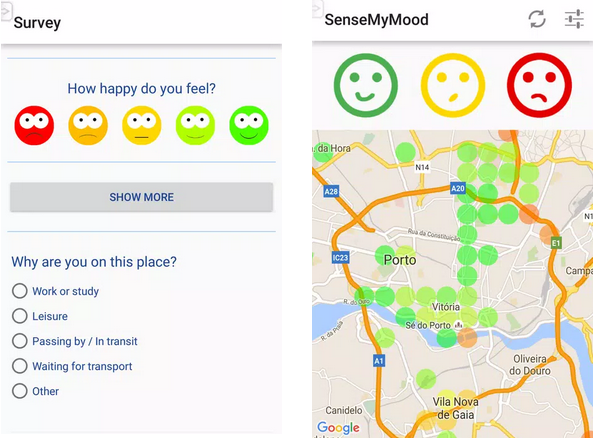
\includegraphics[width=.5\linewidth]{img/SenseMyMood.png}
  \caption{SenseMyMood smartphone application.}
    \label{fig:sensemymood}
    \vspace{-0.5em}
\end{figure}
\noindent \newline One drawback of such approach is the restricted data collection as this application has to be installed explicitly by the user. Therefore only data of persons using this application is processed. An example how to soften this constraint is proposed in (cite) where geo-tagging from social networks such as Twitter, Flickr, Instagram and Facebook is used. Here, text mining algorithms collect the citizens’ emotion from postings. Therefore, all people contribute to the data collection who add the current location to their posts. Nevertheless, smartphone applications have the disadvantage that displaying e.g. the average mood is restricted to users of the application. Last but not least, such map visualizations quickly become overloaded with information when the average mood is displayed for all possible locations in a city.

\subsection{Facade Projection Approaches}
Apart from very few smartphone applications, we only have found some art installations using colored light on building facades as projections for emotions. One example is the project called "Emotional Cities". It was created in 2007 by the artist Erik Krikortz \cite{krikortz_2009} and is an international web art project connected to the public space via light installations. This project was implemented for the city of Stockholm first and continued in Seol later. Here, citizens were able to share their emotions via a web interface by selecting emojis. The Haymarket skyscrapers in Stockholm changed then their color accordingly. The building facades thus act as projections of the average citizens’ mood (see \textbf{figure \ref{fig:emotionalcities}}). The scale ranges from depressed, which is reflected in deep purple, to happy, which is represented in bright red.
\begin{figure}[h]
  \centering
  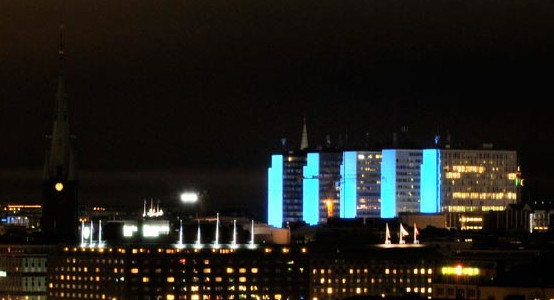
\includegraphics[width=.6\linewidth]{img/bg_emoCities_cutout.jpg}
    \caption{Haymarket skyscrapers in Stockholm reflecting the average citizens’ mood \cite{krikortz_2009}}
    \label{fig:emotionalcities}
    \vspace{-0.5em}
\end{figure}
\noindent \newline With such color projections, however, it is difficult to understand the meaning of individual colors without having further information (it is not clear what e.g. a green facade expresses only by looking at it). Furthermore, the web interface was accessible to everyone, i.e. everyone could submit their emotions - the data did not necessarily correspond to the actual citizens’ mood.

%%%%%%
% Manfred

\begin{figure}[tb]
\centering
\begin{minipage}{.44\textwidth}
  \centering
  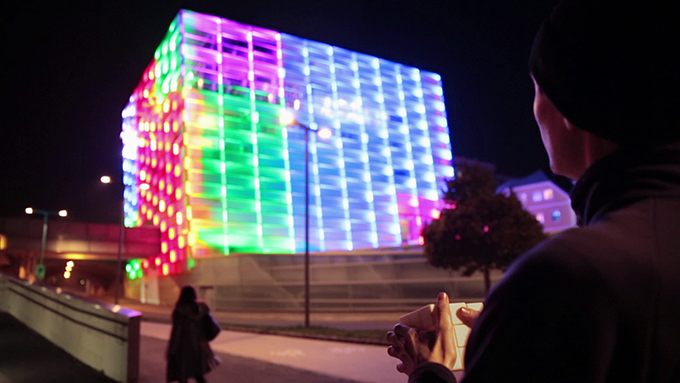
\includegraphics[width=0.8\linewidth]{img/puzzle_facade_web.jpg}
  \caption{Puzzle Facade (AEC Linz) \cite{Lloret2014}}
  \label{fig:puzzlefacade}
\end{minipage}%
\begin{minipage}{.56\textwidth}
  \centering
  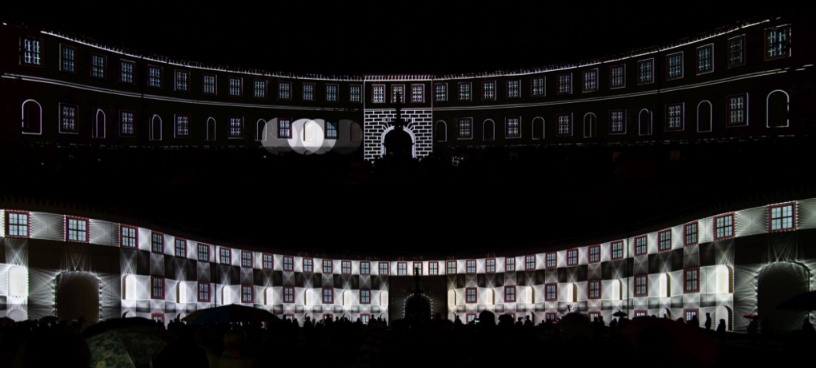
\includegraphics[width=0.8\linewidth]{img/castle_sized_interface.png}
  \caption{Castle-Sized Interfaces \cite{Fischer2015}}
  \label{fig:castlesizedinterface}
\end{minipage}%
\vspace{-1em}
\end{figure}


To improve expressiveness beyond the display of simple colors, we need to look at more sophisticated facade projection projects that were not specifically designed to express emotions.

One step forward is the interactive facade of the Ars Electronica Center (AEC) in Linz, Austria which was put in operation in 2009 \cite{Aec2009}.
Here the facade of the building is divided into segments, each equipped with RGBW LED bars.
These LED bars can be individually controlled in color and brightness via a real-time capable bus infrastructure.
Thus, the entire facade can be used as a low-resolution, responsive display.

The facade is used for various visualization projects and also to highlight events in the city of Linz.
An early example of an interactive installation was "play the facade" from 2009 \cite{Aec2009}, where visitors could connect their cell phones to the facade and visualize their music.
A more recent example was "Puzzle Facade" from 2014 \cite{Lloret2014}, where the facade was turned in a giant Rubik’s cube game controllable by a cube-like tangible interface (see \textbf{figure \ref{fig:puzzlefacade}}).

What is particularly remarkable about the AEC facade is that it has been in continuous use since 2009.
This shows that a permanent installation of this type is possible, which is an important aspect in our case study.

Even more expressive visualizations can be realized using using projection- or video mapping.
Projection mapping uses high-resolution projectors with high light intensity to project still or animated images onto real 3D objects \cite{Dalsgaard2011}.
The images are distorted beforehand so that they correspond to the geometric structure of the object.

One example for the use of such a mapping technique at a big-scale was "Castle-Sized Interfaces" at the castle Elisabethenburg in Meiningen in 2014 \cite{Fischer2015}.
In this installation, the whole facade of the castle was used as a surface for projection (see \textbf{figure \ref{fig:castlesizedinterface}}).

Besides the large scale of the installation, the interactive aspect was another highlight.
By pulling on a rope stretched between bicycle wheels, visitors could move objects within the projection.
Particularly noteworthy here is that the projection had to be rendered in real time so as not to disrupt the impression of immediate interaction.

Although, such an approach provides a considerably higher degree of freedom and expressiveness in contrast to other solutions, it is also very complex and seems less robust.
Special considerations must be made to create a durable and robust projection mapping installation as required for our case study. To help with the decision of finding a fitting approach we can draw from the findings of Dalsgaard et al \cite{Dalsgaard2010} and Parker et al  \cite{Parker2020}. The papers draw conclusions from multiple real world public interactive displays. Those findings will help us achieve a more robust and approachable design by providing experiences from various implementations of public interactive displays.
%%%%%%


%%
%% The acknowledgments section is defined using the "acks" environment
%% (and NOT an unnumbered section). This ensures the proper
%% identification of the section in the article metadata, and the
%% consistent spelling of the heading.
%\begin{acks}
%To Robert, for the bagels and explaining CMYK and color spaces.
%\end{acks}

%%
%% The next two lines define the bibliography style to be used, and
%% the bibliography file.
\bibliographystyle{ACM-Reference-Format}
\bibliography{sample-base}

%%
%% If your work has an appendix, this is the place to put it.
%\appendix

\end{document}
\endinput
%%
%% End of file `sample-manuscript.tex'.
